\section{Visualization Verification}
Our proposal is to recognize and verify the presentation of various graphical domain-specific languages. As an intermediate step for the first proof of concept\footnote{A demonstrator for this proof of concept is available on: https://gitlab.com/domaines}, we start with a single view of one graphical domain-specific language. 
The Open Avionics Architecture Model (OAAM) \cite{Annighoefer2019} is an ecore-based metamodel for modeling avionics systems. This model comprises multiple layers, with our attention directed towards the functions layer, which describes function logics and data flow. The function is broken down into atomic tasks. These tasks can be sensors, actors, routings, or logics. They have ports (input and output) that can be connected with signals.

\begin{figure}[htb]
  \centering
  \includegraphics[width=\linewidth]{figures/visualization_model_functions_print_ink.pdf}
  \caption{A subset of the editor model of \cite{Annighoefer2021} showing the visualization model for the OAAM functions editor}
  
  \label{fig:visualization_model_functions}
\end{figure}

To elucidate our approach, we employ a minimalistic model of a \emph{Door System} as a running example. 
The visualization of our models is implemented using XGEE \cite{Annighoefer2021}, a web-based graphical model editor that leverages an editor model to facilitate both visualization and interaction. The editor model allows defining editors for ecore models in a model-driven way. Both visualization and interaction are modeled. For the block diagram recognition, we leverage the visualization part, which we call the visualization model. It composes the visualization out of the basic elements: vertex, edge, and label. They can be arranged hierarchically and represent model elements that are retrieved by a query in the Essential Object Query (EOQ) \cite{Annighoefer2019} language. Vertices are graphics like \emph{task.svg}. The object diagram is depicted in \autoref{fig:visualization_model_functions}. It shows the two top-level elements: task and signal. While a task is a vertex and can be freely positioned, the signal connects two ports, which are attached to vertices. Tasks and ports have labels. 

\begin{figure}[htb]
  \centering
  % \includegraphics[width=\linewidth]{figures/door_system_xgee_untouched.png}
  \includegraphics[width=\linewidth]{figures/door_system_xgee_untouched_big.png}
  \caption{Screenshot of XGEE using the Functions Editor model to visualize the demo use case Door System}
  
  \label{fig:door_system_xgee_untouched}
\end{figure}

The \emph{Door System} model includes basic tasks representing the opening and closing buttons, a control logic, and lights showing the status, all visualized through XGEE. A screenshot is depicted in \autoref{fig:door_system_xgee_untouched}. 
We have defined 14 test cases simulating visualization errors. The test cases comprise errors related to vertices, edges and labels, covering incorrect, not enough, and too many visualizations. The test cases are depicted in \autoref{tab:test_cases} and \autoref{tab:test_cases_text}; their results are discussed in Section \ref{sec:results}. As a running example for explaining the methodology, we use the test case \emph{task too small}, because it triggers error indications in all steps. In this case, the box of \emph{Task Actor Unlocked} in the \emph{Door System} is shrunk such that it is no longer clearly visible as a task. 

\subsection{Overview Visualization Verification Approach}

The overall visualization verification process is illustrated in \autoref{fig:recognition_overview}. A screenshot is taken, in which the XGEE modeling canvas is located and clipped. User interface artifacts are removed. The screenshot is then tokenized using lexical grammar to break down the visual elements into recognizable tokens. Following this, a hierarchical structure is reconstructed based on the positioning syntax.
Subsequently, the recognized model is instantiated. Only the model itself is relevant; the layout is not retrieved.  This instantiated model is then compared to the original model to identify relevant discrepancies. Visualization errors can be detected at four main steps of this process: tokenization, syntactical analysis, model instantiation, and model comparison. 

If the model is correctly visualized, the visualization verification does not find any discrepancies. The user can now be sure that the block diagram correctly depicts the model and continue with further processing. If visualization errors are found, they are communicated to the user. Errors detected during tokenization and syntactical analysis, which are associated with specific image areas, can be visualized in the model visualization. They are depicted as red bounding boxes on an overlay. In contrast, visualization errors detected during model instantiation and model comparison are not directly linked to image areas and cannot be visualized. These visualization errors are instead reported in a textual report. 


\begin{figure*}[htb]
  \centering
  \frame{\includegraphics[width=\linewidth]{figures/overview_2_3_tex.pdf}}
  \caption{Steps of the visualization verification process}
  
  \label{fig:recognition_overview}
\end{figure*}


\section{Block Diagram Recognition}
Edges represent connections between vertices, inputs and outputs. Detecting edges accurately requires an approach that can identify individual line segments and how they connect to form complex chains. This section introduces a robust edge detection pipeline leveraging multiple computer vision techniques to reliably identify edges across a wide variety of block diagrams within XGEE. 

\subsection{Preprocessing}

% latex really wants this graphic on the next page...
\begin{figure}[htb]
  \centering
  \frame{\includegraphics[width=\linewidth]{figures/door_system_after_preprocessing_big.png}}
  \caption{Plain block-diagram after preprocessing}
  
  \label{fig:preprocessing}
\end{figure}

The process starts with a screenshot. To make the process as user-friendly as possible, we avoid the need to configure the location of the XGEE window. This is achieved by taking a screenshot of all screens. Within this large screenshot, pixels with the distinct color of the XGEE title bar and status bar are identified. The bounding box of these pixels defines the XGEE window. Afterward, the image is thresholded to find white and near-white areas. The largest white contour is the modeling canvas. Since the grid is convenient for users, but not relevant for the model, it is removed by replacing the distinct grid colors with white. Similarly, the tools in the corners of the canvas are replaced with white. The output of preprocessing is the plain block diagram on a white canvas, as depicted in \autoref{fig:preprocessing}.


\subsection{Tokenization}
The first step of the recognition process is tokenization. In this process, each vertex, edge, and label is treated as a distinct token, allowing for separate identification. Overlapping tokens, such as ports, are possible. For the OAAM Functions Editor, the tokens are as follows. Large blue boxes defined in \emph{task.svg} depict tasks. Tasks can have input ports and output ports which are depicted as white and black triangles from \emph{output.svg, input.svg}, respectively. Edges represent signals and connect outputs to inputs. Text elements are labels. The necessary information is available in the visualization model. Analogous to a textual parser, we call the mapping of graphic to token type \emph{lexical grammar}. 

The objective of tokenization is to identify token types from the lexical grammar and their positions within the preprocessed screenshot. For two-dimensional token types (\emph{task, input, output, text}), the bounding boxes are determined. For edges (\emph{signal}), the polygonal chain and its width are extracted. Ultimately, the aim is to discern which pixels correspond to a token type and which do not.
% TODO text more paper style. 

\subsubsection{Resizable vertices}
First, we identify resizable vertices within the model. In our DSL, this involves using template matching with a provided \emph{task.svg} token type. Tasks are resizable to accommodate additional ports and for aesthetic layout purposes. This approach leverages Normalized Cross-Coefficient Matching, as described in \cite{Lewis1995}. $I$ represents the image, which is  the preprocessed screenshot,  $T$ denotes the template, the \emph{task}, and  $R$ is the result. 

% first try
% \begin{equation}
%   R(x, y) = \frac{\sum_{x', y'} \left( T(x', y') - \bar{T} \right) \left( I(x + x', y + y') - \bar{I}(x, y) \right)}{\sqrt{\sum_{x', y'} \left( T(x', y') - \bar{T} \right)^2 \sum_{x', y'} \left( I(x + x', y + y') - \bar{I}(x, y) \right)^2}}
% \end{equation}.

% from opencv manual: https://docs.opencv.org/4.10.0/df/dfb/group__imgproc__object.html#ga3a7850640f1fe1f58fe91a2d7583695d
\begin{equation}
  R(x, y) = \frac{\sum_{x', y'} \left( T'(x', y') \cdot \left( I'(x + x', y + y')  \right) \right)}  {\sqrt{\sum_{x', y'}  T'(x', y')^2 \cdot \sum_{x', y'}  I'(x + x', y + y') ^2}}
\end{equation}
where

\begin{equation*}
    T'(x', y') = T(x', y') - \frac{1}{(w \cdot h)} \sum_{x'', y''} T(x'', y'')
\end{equation*}

\begin{multline*}
    I'(x + x', y + y')  = I(x + x', y + y') - \frac{1}{(w \cdot h)} \sum_{x'', y''} I(x + x'', y + y'')
\end{multline*}


We use the implementation in the Python library OpenCV \cite{Bradski2000}.

\begin{figure}[htb]
  \centering
  % \includegraphics[width=\linewidth]{figures/door_system_template_matching_task.png}
  \includegraphics[width=\linewidth]{figures/vertices_overlay_clip_big.png}
  \caption{Plot of the normalized cross correlation between preprocessed screenshot \emph{Door System} and template \emph{task}}
  
  \label{fig:door_system_template_matching_task}
\end{figure}

For each potential position, the similarity between the template and the current patch of the screenshot is calculated and normalized to a range from -1 to 1.

The correlation results are visualized in a 3D plot in \autoref{fig:door_system_template_matching_task}, with the highest correlation values around 90\% indicating a successful match. A coordinate system with the origin at the top left is used, which is why the unscaled \emph{Task Door System Logic} is identified as a spike at its top left. Other boxes are scaled: \emph{Task Sensor Open Button} and \emph{Task Actor Locked} along the x-axis, and \emph{Task Sensor Close Button} along both the x and y axes. This results in correlation spikes appearing as lines or rectangles rather than discrete points.
A threshold for minimal correlation is used. Lines and rectangles are grouped into larger rectangles. These groups represent one task each. In our running example \emph{task too small}, we can see that the \emph{Task Actor Unlocked} at the bottom right is not detected, as expected.

\subsubsection{Fixed-size vertices with transparency}
In the OAAM Functions Editor, black and white right-pointed triangles represent inputs and outputs, and they are characterized by their fixed size. However, a significant challenge arises due to their overlap with tasks. As depicted in \autoref{fig:door_system_xgee_untouched}, they are partially on the background and partially on a task. Additionally, inputs and outputs may be used for other boxes with different colors. Therefore it is not enough to search for a rectangular patch; we need to search for the precise triangle form of ports independent of the background. 

To address this, we utilize normalized squared differences with the mask $M$ for treating transparency.


\begin{equation}
    R(x, y) = \frac{\sum_{x', y'} \left( \left( T' - I(x + x', y + y') \right)  \cdot M' \right)^2}
{\sqrt{\sum_{x', y'} \left( T'  \cdot M'\right)^2 
\cdot \sum_{x', y'} \left(  I(x + x', y + y') \cdot M'     \right)^2
 }}
\end{equation}

where
\begin{equation*}
T' = T(x', y'), \quad M' = M(x', y')    
\end{equation*}



By incorporating transparency into the correlation calculations, we can precisely locate ports. 
The result is shown in \autoref{fig:door_system_template_matching_input}. The matches produce distinguishable spikes. 

\begin{figure}[htb]
  \centering
  \includegraphics[width=\linewidth]{figures/ports_overlay_clip_big_nls_clip.png}
  \caption{Plot of the squared differences between of preprocessed screenshot \emph{Door System} and template \emph{input}}
  \label{fig:door_system_template_matching_input}
\end{figure}

\subsubsection{Edges}
Edges represent connections between vertices, inputs and outputs. Detecting edges accurately requires an approach that can identify individual line segments and how they connect to form complex chains.

To detect edges, we employ a kernel-based detection method. This involves applying a kernel function specifically designed to identify horizontal and vertical lines composed of a sequence of colors (white,black, white) with predefined widths. The kernel function convolves the image with the kernel to detect these patterns.
Raw results for detecting horizontal lines are depicted in Figure \ref{fig_filter2d}.
A threshold is applied to ensure that the detected lines correspond to the edges rather than the black lines used in task boxes.
As illustrated in figure \ref{fig_misidentified_edges}, inputs and outputs are sometimes misidentified as edges. Additionally, intersections of edges and points where horizontal and vertical edges meet are not immediately detected. These challenging areas will be processed individually in a later step in the edge detection pipeline. Apart from these specific cases, the method effectively extracts all pixels corresponding to vertical and horizontal edges, provided their widths match those of the used kernels.

\begin{figure}[htb]
  \centering
  \includegraphics[width=\linewidth]{figures/filter2D.png}
  \caption{Plot of the convolution between between preprocessed screenshot Door System and horizontal edge kernel}
  \label{fig_filter2d}
\end{figure}

For easier processing and data storage, the thresholded pixels are converted to line segments consisting of start- and endpoints.

\begin{figure}[htb]
  \centering
  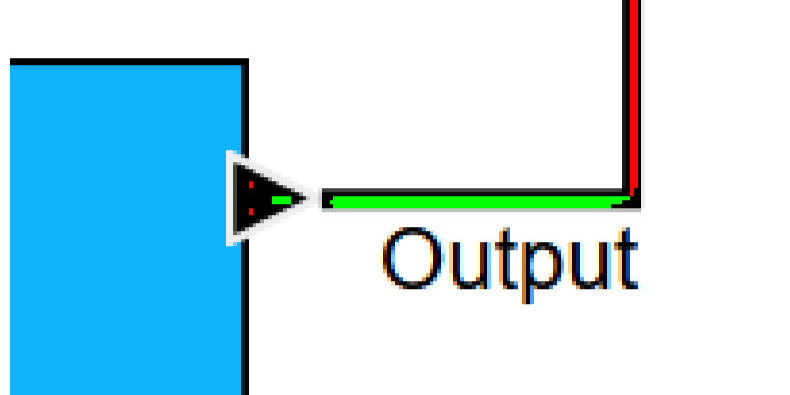
\includegraphics[width=\linewidth]{figures/thresh_zoom.png}
  \caption{Detected vertical and horizontal pixels around an output before filtering short segments}
  \label{fig_misidentified_edges}
\end{figure}

Misidentified letters and ports are removed by filtering out all line segments with a length shorter than 20 pixels. In all test cases, this approach successfully removes the unwanted line segments while keeping the edges, illustrated in figure \ref{fig_comparison_filter}.
As shown in figure \ref{fig_threshold}, the \textit{filter2D()} function initially does not detect any edges at intersections, leading to gaps between the line segments. To process these gaps, it is assumed that intersections always consist of two straight edges. Overlapping 90$^{\circ}$ turns are considered impossible and will result in an error caused by the incorrect edge recognition. This forces the user to maintain a clear diagram structure.
First, all intersections in the image are detected using OpenCV's \textit{matchTemplate()} function, which matches a template image to overlapping regions of the target image \cite{web_matchTemplate}.
The function slides the template across the image, comparing overlapping patches with the template using a specified method. Among the available methods \cite{comparison_methods}, tm\_sqdiff\_normed produced the most accurate results. For each pixel, the function calculates and assigns a value representing the similarity between the template and the corresponding image region below. While this approach is more precise than \textit{filter2D()}, it is also significantly more resource-intensive.
% \begin{equation}
% \label{tm_sqdiff_normed}
%     R(x,y) = \frac{\sum_{x', y'}{(T(x', y') - I(x + x', y + y'))^2}}{\sqrt{\sum_{x', y'}{(T(x', y')^2 * \sum_{x', y'}{I(x + x', y + y')^2}}}}
% \end{equation}
At intersections, the similarity value is approximately 85\%. This slight discrepancy likely arises from how modern operating systems use aliasing to render text and lines with higher apparent resolution and contrast compared to the display. Zooming in reveals that the white pixels near edges are often replaced with subtle color hues or shades of gray. Rendering the results of the template matching highlights a peak in similarity at the intersection (Figure \ref{fig_intersection_peak}). Thresholding isolates this peak, typically yielding two or more matches per intersection. These matches are then filtered based on proximity, ensuring only one match is detected at each intersection.

\begin{figure}
    \centering
    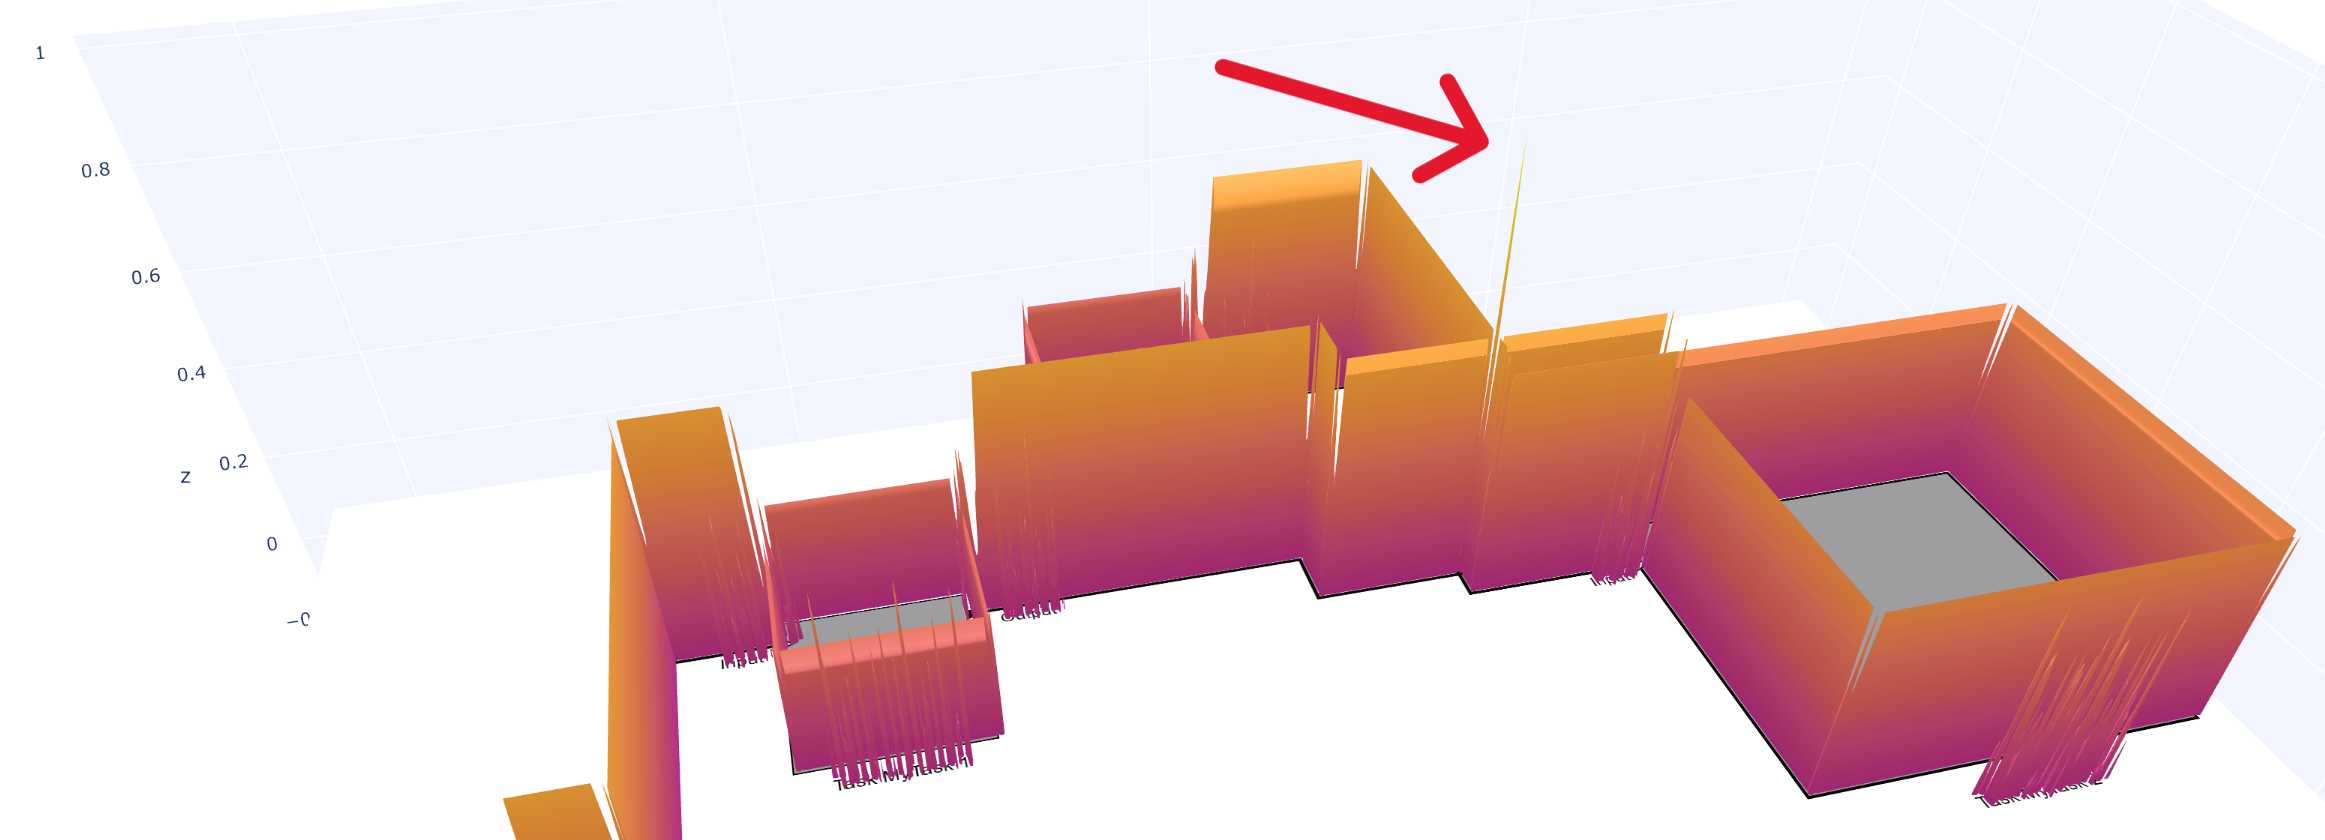
\includegraphics[width=1\linewidth]{figures/intersection_peak.png}
    \caption{Simmilarity score is high at edges and vertex borders, but peaks at intersections. (visualized in 3d using \textit{plotly}).}
    \label{fig_intersection_peak}
\end{figure}

The method then processes each detected intersection by connecting the two vertical and two horizontal line segments. This eliminates any residual points near the intersection, leaving only one vertical and one horizontal line segment, illustrated in figure \ref{fig:_intersection_before_after}.
In the allocations editor, the same approach is applied to detect and process signal containers on edges. To enhance diagram readability, it is assumed that no 90$^{\circ}$ turns are concealed behind the containers and that edges pass through them in a straight line, avoiding ambiguities that could confuse both computer vision algorithms and human users. The primary distinction from intersection detection lies in the number of line segments: at a signal container, only two line segments meet, rather than four.
\begin{figure}[h]
    \centering
    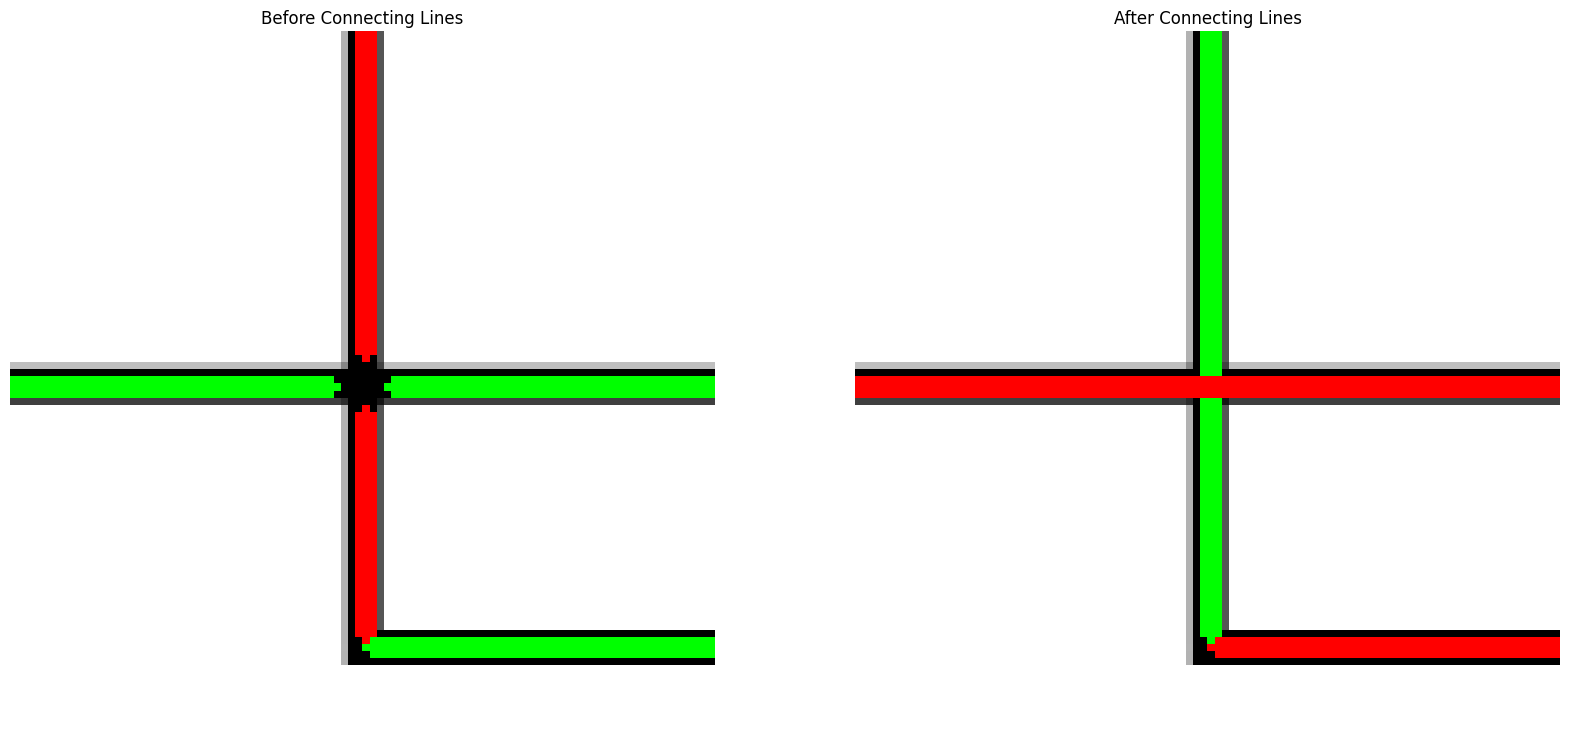
\includegraphics[width=0.7\linewidth]{figures/intersection_before_after.png}
    \caption{Intersection before and after connecting the line segments.}
    \label{fig:_intersection_before_after}
\end{figure}
Converting the line segments into polylines at this stage would produce unusable data, as the segments are not grouped and not sorted in the sequential order of the edge's \textit{flow}. To generate proper polylines, the line segments must first be sorted into the correct order. For instance, if the first line segment in the list is an intermediate segment within an edge, the polyline function may mistakenly attempt to connect its endpoints directly to the next point in the list, without considering whether it belongs to the same continuous chain, resulting in incorrect edge detections.
The implemented method begins by selecting the first line segment, adding it as a starting point to the first chain and to a list of used segments and setting the \textit{chain\_growing} flag to true. It then iterates through the remaining segments, checking whether each segment has already been used and whether any of its points lie within 7 pixels of the endpoints of the current segment. If a match is found, the segment is added to the \textit{used\_segments} list and the current chain. If no segment is found within the 7-pixel threshold, the \textit{chain\_growing} flag is set to false, and the completed chain is added to the list of chains. A threshold of 7 pixels was selected as it reliably produces connected polylines while ensuring that closely positioned lines, such as those at ports, remain distinct and seperate. This process continues until all line segments have been assigned to a chain as in figure \ref{fig_chains_before_after}.
\begin{figure}[h]
    \centering
    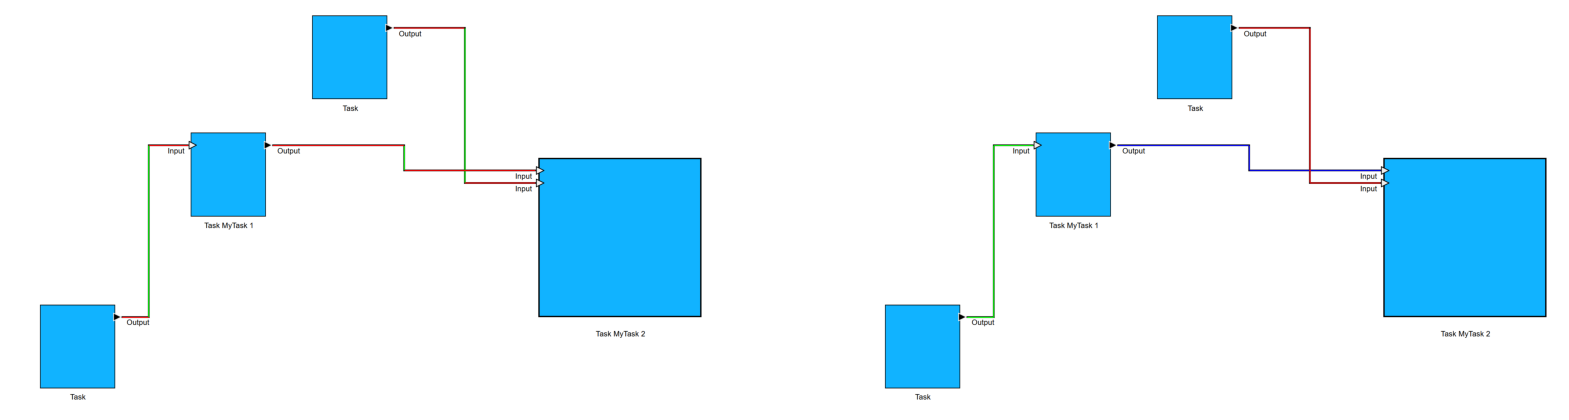
\includegraphics[width=\linewidth]{figures/chains_before_after.png}
    \caption{Left: detected vertical and horizontal line segmentsRight: detected line segments grouped into colored line segment chains}
    \label{fig_chains_before_after}
\end{figure}
Generating the polylines now would yield better results, but still create unusable data, because the line segments within each chain and the two points within each line segment are not sorted. The first point in a list of line segments in a chain could for example be a point in the middle of the chain, resulting in OpenCV's Polyline function to connect the following points in the wrong order.
The sorting algorithm for solving this problem consists of two steps: the first sorts the line segments from the beginning of the chain to the end, the second sorts the end- and startpoint of each line segment individually, so that they too appear in sequential order of 'flow' in the chain.
To distinguish between intermediate points and endpoints, the function relies on the method by which the points were initially identified: when two line segments intersect to form a 90$^{\circ}$ degree turn, each segment consists of a start- and an endpoint. As a result, intermediate points in a chain, where line segments meet, always have two points in close proximity, whereas endpoints only have a single point, since only one line segment terminates at each endpoint (see Figure \ref{fig_point_zoom}).
The function leverages this discrepancy by identifying endpoints through an iterative process: It examines each point and checks for the presence of other points within a seven-pixel radius. If no other points are found within this radius, the point is classified as an endpoint of a chain.
\begin{figure}
    \centering
    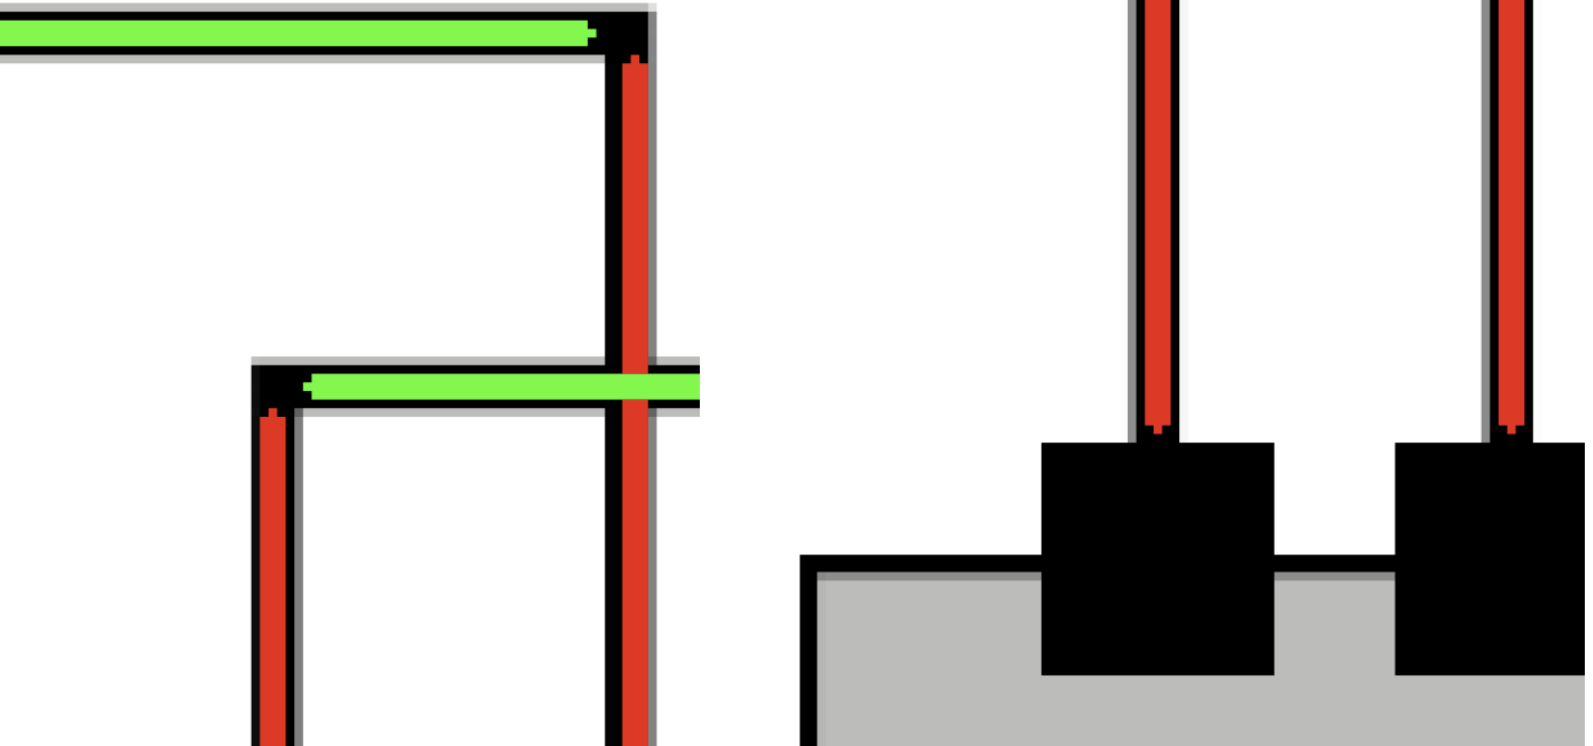
\includegraphics[width=0.5\linewidth]{figures/zoomed_in_points.png}
    \caption{Difference between intermediate points and endpoints}
    \label{fig_point_zoom}
\end{figure}
Using the identified endpoints to initialize the \textit{sorted\_chain} list allows the program to organize the chains systematically. The process begins by selecting the segment that includes one of the start points as the initial segment of the chain. The endpoint of this segment that is not a chain endpoint is designated as the first \textit{last\_point} in the \textit{sorted\_chain} list. To determine the next segment in the chain, a \textit{lambda function} calculates the distance between the last point and both points of each remaining segment. The segment containing the point with the smallest distance to the \textit{last\_point} is selected as \textit{next\_segment} and removed from the list of \textit{remaining\_segments}. Within this segment, the point closest to the \textit{last\_point} is appended first to the \textit{sorted\_chain}, followed by the other point of the segment. This process repeats until no segments remain in the \textit{remaining\_segments} list. The entire process is repeated for each chain until all points in all chains are ordered according to the edge's \textit{flow}.

Polylines, which represent connected line segments as ordered lists of points, are a fundamental component in reconstructing edges within the diagram. To generate these polylines from the sorted chains, the method iterates through the \textit{sorted\_chains} list, sequentially appending each point to construct the polylines.The preprocessing of the data ensures that the chains are already structured correctly, making the generation of polylines straightforward and efficient. Once the polyline is constructed, it is converted into the format required by OpenCV for further processing.

\subsubsection{Text}
To identify text within the model, we utilize Tesseract \cite{Smith2007}, an open-source optical character recognition (OCR) engine. Tesseract operates in a mode optimized for sparse text, which is suitable for the typical distribution of text in our models.

One challenge is that in larger diagrams, Tesseract may incorrectly detect large blocks as hyphens or other characters. To address this, we apply filters based on the known font size. 
Additionally, Tesseract provides a confidence metric for each detected text element. This metric indicates the engine's certainty regarding the correctness of the detected text. We utilize this confidence score to ensure that only highly confident detections are retained for further processing. Specifically, we employ a two-step approach: text blocks with confidence levels below 80 are completely filtered out, while those with confidence levels between 80 and 90 trigger a warning, prompting the user to check the labels. 
In our running example, the bounding boxes and contents of all texts are correctly recognized. Together with all other detected tokens, the text boxes and their contents are visualized in \autoref{fig:detected_model_elements}.

\subsubsection{Untokenized areas}
The result of the tokenization steps for the \emph{task too small} test case is depicted in \autoref{fig:detected_model_elements}. For all detected tokens, it shows bounding boxes or polygonal chains. As expected, the bounding boxes of ports and tasks overlap.  In the next step, the positions of these bounding boxes and their corresponding token types will be utilized. 

At this step, first visualization errors can be detected. It is possible to analyze untokenized areas. When comparing the foreground with the tokenized elements, the \emph{Task Actor Unlocked} is detected as untokenized and reported as a visualization error. This is shown as \emph{untokenized pixels} in \autoref{fig:door_system_xgee_vvt}. The actual error is that the box is too small, but it can only be reported that there are pixels that do not match any token type.

\begin{figure}[htb]
  \centering
  \frame{\includegraphics[width=\linewidth]{figures/detected_model_elements_big.png}}
  \caption{Detected model elements with token type and bounding box of the \emph{Door System}, overlayed on the preprocessed screenshot}
  
  \label{fig:detected_model_elements}
\end{figure}

\subsection{Positioning Syntax and Hierarchy Retrieval}
The visualization model specifies the positioning of elements within the diagram. We call positioning rules \emph{Positioning Syntax}. Top-level vertices, such as tasks, can be freely positioned. However, inputs are restricted to the left side of tasks. The position of text labels is also defined: they must be to the left of inputs, to the right of outputs, or at the bottom of tasks. 
Edges are treated differently. In this model, edges are only permitted between outputs and inputs, meaning their endpoints are strictly defined. The Positioning Syntax is checked for each model element to ensure proper positioning and report visualization errors. 

Using these rules, a hierarchical structure is reconstructed. Model elements that are positioned incorrectly are reported as visualization errors. In our running example \emph{task too small}, the text label \emph{Task Actor Unlocked} is flagged as a visualization error because it lacks a parent element; the associated task was not detected. Conversely, the label \emph{Input} is correctly positioned to the left of an input. However, the \emph{input} triangle itself is reported as an error since there is no task tokenized to its right.


\subsection{Model Instantiation}
Using the visual hierarchical relationships established in the previous step, an abstract syntax tree (AST) is instantiated. This AST serves as the foundation for the instantiation of the recognized model. The visualization model provides the mapping between token types and class names.
For example, an image file named \emph{task.svg} is mapped to the class Task. Similarly, labels are typically instantiated as the name attributes of objects. Signals are also instantiated, with their endpoints defined as attributes.

\begin{figure}[htb]
  \centering
  \includegraphics[width=\linewidth]{figures/door_system_xgee_recognized.png}
  \caption{Visualization of the model reconstructed from the recognized elements}
  
  \label{fig:door_system_xgee_recognized}
\end{figure}

The visualization of the instantiation for our running example \emph{task too small} is depicted in \autoref{fig:door_system_xgee_recognized}. As can be seen from the results, most elements are recognized correctly. However, the differences are.
Firstly, the task \emph{Actor Unlocked} is missing from the detected elements. This omission also leads to the absence of its input and the signal connecting its output to its input. This is as intended since the task in the original model is too small. Without the parent, it is not possible to instantiate the correctly detected \emph{Input}. This problem propagates; the correctly detected signal cannot be connected to an uninstantiated \emph{Input}, which triggers an instantiation error. 

Further details of the block-diagram recognition process can be observed. The task boxes are all displayed at their default size; in other words, their individual size is not reconstructed. Furthermore, the open button is now above the close button; this is inverted in comparison to the original model. This shows that positioning is also not reconstructed. 
These differences are only in the layout. Since the information about what box is where is retrieved, the layout could be reconstructed. However, the current focus is visualization verification, hence reconstruction is not considered. 

\section{Compare Recognized Model and Visualize Results}
The model of the block diagram is now fully recognized. In the next steps, the recognized model is compared to the original model. The resulting error indications are presented in the user interface. 


\subsection{Model Comparison}
The final step of model visualization verification is comparing the recognized model to the original model. There are sophisticated model comparison algorithms available, such as \cite{Brun2008}. For the time being, the original model and the recognized model are compared in a fairly simple way using EOQ queries. 
Firstly, the quantity of tasks is compared. Then the labels of tasks are compared to retrieve a mapping of the tasks between original and recognized model. 
Afterward, the signals are compared. Signals are compared using the labels of input, input task, output, and output task.

In our running example \emph{task too small}, model comparison detects two errors: the task \emph{Actor Unlocked} and the signal \emph{Door System Logic:Output - Actor Unlocked:Input} are missing in the recognized model. 


\subsection{User Interface}
To enable the user to address the visualization problem, it is communicated through the user interface.
The detected visualization errors are presented to the user in two ways: through graphical error indications and textual error descriptions.

% \subsubsection{Graphical Error Indication}
To visualize error indications, an error indication layer is introduced on top of the Functions Editor. The visualization errors from the steps tokenization and syntactical analysis are directly related to pixels in the image whose bounding box is known. Therefore, a red bounding box with a description label is overlaid on the problematic areas. In the case of our \emph{Door System}, the tokenization detects the too small blue box as untokenized pixels. Without a \emph{Task}, the \emph{Task label} breaks the syntax rules and is highlighted, too. The same applies to the \emph{Input}. The graphical error indication is depicted in \autoref{fig:door_system_xgee_vvt}.
The three visualized errors clearly indicate the source of the problem. However it is now up to the user to find out that the task box is too small. 

\begin{figure}[htb]
  \centering
  \includegraphics[width=\linewidth]{figures/door_system_xgee_vvt_big.png}
  \caption{Graphical report of the visualization errors through error boxes}
  
  \label{fig:door_system_xgee_vvt}
\end{figure}

% \subsubsection{Textual Error Indication}
The visualization errors from the steps model instantiation and model comparison cannot be graphically highlighted. For these errors, a textual report is generated. The report is shown directly in XGEE as depicted in \autoref{fig:door_system_xgee_vvt_error_report}. For the sake of completeness, the error indications that are already highlighted with a red box are additionally added to the textual error report. 

\begin{figure}[htb]
  \centering
  \includegraphics[width=\linewidth]{figures/door_system_xgee_vvt_error_report_clip.png}
  \caption{Textual report integrated in the GUI of XGEE}
  
  \label{fig:door_system_xgee_vvt_error_report}
\end{figure}



    